\section{Seguimiento}

Los puntos obtenidos para todos los cuadros luego de la reconstrucción deben ser identificados en trayectorias temporales a lo largo de la secuencia.


El seguimiento de trayectoria se realiza sobre una ventana deslizante de tres a cuatro cuadros donde se enlazan los puntos reconstruidos de manera de mantener un movimiento lo mas suave posible debido a la hipótesis que el muestreo permite observar una evolución lenta con desplazamiento mínimo entre cuadros.


Esta metodología fue la utilizada por Herda \cite{herda} en su trabajo basándose en los estudios de Malik, Drako, Papantoniou \cite{griegos} .

\subsection{Algoritmo}

Sea una trayectoria de un marcador enlazada hasta el instante [f] la cual desea buscarse su próximo punto en [f+1], el movimiento entre [f-1] y [f] es prolongado en dirección y modulo para establecer un centro de búsqueda para encontrar el punto reconstruido que mejor continúa la trayectoria en un proceso mostrado en la Figura \ref{herda_00} .

\begin{figure}[ht!]
\begin{center}
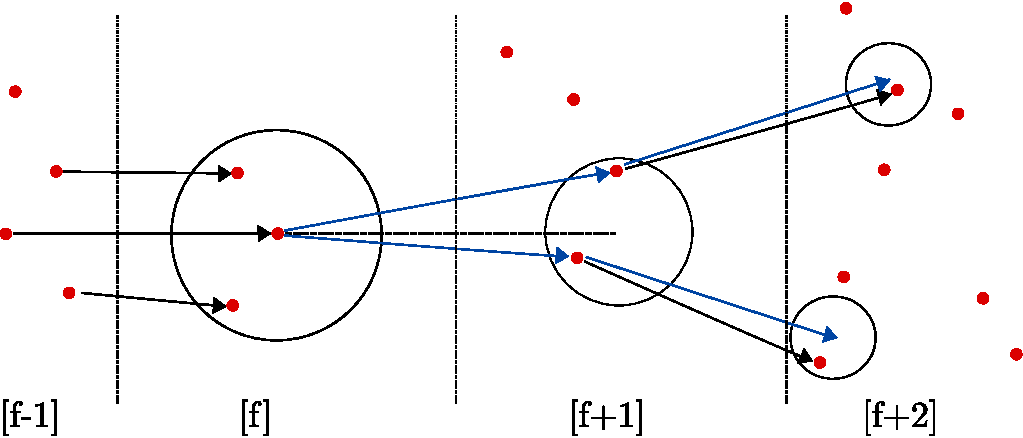
\includegraphics[scale=0.8]{imagenes/Seguimiento/tracking-eps-converted-to.pdf}
\end{center}
\caption{Seguimiento en cuatro cuadros, siendo [f] el cuadro actual que queremos seguir en [f+1]. ( Fuente  Human movement
science 20(3), 313–341 \cite{herda} ) .}
\label{herda_00}
\end{figure}

Se presentan tres posibles casos al buscar puntos reconstruidos:

\begin{itemize}

\item Si solo se encuentra un punto reconstruido dentro de la búsqueda se agrega a la trayectoria para el cuadro [f+1], mientras mas cercano se encuentre a la estimación calculada en la Ecuación \ref{centro_busqueda_f1} mejor se aproxima a una trayectoria de tres puntos con aceleración mínima

\begin{equation}
\begin{split}
\boldsymbol{\overrightarrow{v}}_{[f][f+1]}^{i} = \boldsymbol{\overrightarrow{v}}_{[f-1][f]}^{i} \Rightarrow C_{[f+1]}^{i} &= x_{[f]}^{i} + \boldsymbol{\overrightarrow{v}}_{[f-1][f]}^{i}.\Delta{t} \\
&= 2.x_{[f]}^{i} -x_{[f-1]}^{i} 
\end{split}
\label{centro_busqueda_f1}
\end{equation}

\item En el caso de encontrar mas de un punto dentro del radio de búsqueda cada posible candidato es utilizado para realizar una segunda estimación hacia [f+2] de forma que la aceleración entre [f-1], [f] y el candidato en [f+1] sea la misma que entre [f], el candidato en [f+1] y la estimación en [f+2] (el radio de búsqueda en [f+2] corresponde a la distancia entre el candidato en [f+1] y la estimación en [f+2]). Luego de todos los posible caminos en cuatro cuadros, se elige el de menor variación de aceleración.

\begin{equation}
\hspace{-1cm}
\begin{split}
\boldsymbol{\overrightarrow{a}}_{[f][f+1][f+2]}=\boldsymbol{\overrightarrow{a}}_{[f-1][f][f+1]} \Rightarrow C_{[f+2]}^{i} &= x_{[f+1]}^{i} + \boldsymbol{\overrightarrow{v}}_{[f][f+1]}^{i}.\Delta{t} + \boldsymbol{\overrightarrow{a}}_{[f-1][f][f+1]}^{i}.\Delta{t}^2\\
&= 3.x_{[f+1]}^{i} - 3.x_{[f]}^{i} + x_{[f-1]}^{i}\end{split}
\label{centro_busqueda_f2}
\end{equation}

\item Si no se encuentra ningún punto, se procede a aumentar acotadamente el radio de búsqueda en [f+1] de forma excepcional. Esto se hace para continuar trayectorias que entran en estado de reposo y el ultimo movimiento conocido es nulo o muy pequeño.

\end{itemize}

Una vez establecidos posibles enlaces entre las trayectorias encontradas hasta [f] con los marcadores reconstruidos en [f+1], debe validarse cada enlace encontrado de forma que cada punto en [f+1] pertenece a una única trayectoria y en caso que fuese candidato en múltiples trayectorias se utiliza el criterio de menor aceleración para elegir entre trayectoria, donde la trayectoria descartada se enlaza con la siguiente mejor opción obtenida en la búsqueda.

Posteriores validaciones son realizadas sobre el conjunto de trayectorias obtenidas al procesar todos los cuadros de forma opcional: 

\begin{itemize}

\item Validación global donde la aceleración de todos los enlaces obtenidos en todos los cuadros es estudiada mediante distribución estadística, descartando  el porcentaje superior que corresponden a posibles aceleraciones excesivas puntuales que no cumplen la hipótesis de trayectorias suaves con cambios lentos. Este estudio arroja un umbral global que se utilizara para volver a buscar los enlaces para toda la secuencia donde un enlace que supere este umbral sera descartado .

\item Validación individual, es un caso especifico del filtrado de aceleración donde no se busca un umbral global, sino que cada trayectoria obtenida es estudiada para buscar un umbral individual estudiando la distribución de aceleraciones. Si un enlace o una sección de la secuencia supera este umbral, se intenta estimar el o los marcadores que permitan suavizar la aceleración de la trayectoria mediante mínimos cuadrados buscando aquellos puntos que mejor aproximen el movimiento que mantenga aceleración mínima (se mantiene la misma velocidad) y variación de aceleración mínima (se mantiene la misma aceleración)

\end{itemize}

Esta ultima forma de estimar marcadores intermedios no solo se utiliza en el caso de la corrección en la validación de cada trayectoria individual, sino también para estimar marcadores en caso de perdidas durante la búsqueda de enlaces. 

Cuando se realiza la búsqueda de enlaces sobre los puntos reconstruidos pueden aparecer puntos reconstruidos los cuales no pudieron ser asociados a ninguna trayectoria, mientras que también pueden existir trayectorias truncas debido a no poder encontrar posibles enlaces para continuarlas.

Si esto sucede se agrega la trayectoria a una lista de trayectorias truncas al buscar enlaces entre [f] y [f+1], y se prolonga el movimiento de las trayectorias que se encontraban truncas hasta el momento [f-1] o antes de forma de repetir el movimiento por tantos cuadros durante la trayectoria se encuentre perdida. 

Sobre este movimiento prolongado se buscan puntos reconstruidos en su cercanía y en el caso que exista un candidato en un cuadro [$f_{j}$] de una trayectoria perdida en un instante [$f_{i}$] deben estimarse los puntos intermedios durante los cuales la trayectoria se perdió, [$f_{i}+1$], [$f_{i}+2$], ..., [$f_{j}-1$]

{\scriptsize \begin{equation}
\hspace{-0cm}
\left\{
\begin{matrix}
X_{[f_{i}-2]} &-3.X_{[f_{i}-1]} &+3.X_{[f_{i}]} &-\boldsymbol{\tilde{X}_{[f_{i}+1]}} & & & &=0 \\
& X_{[f_{i}-1]} &-3.X_{[f_{i}]} &+3.\boldsymbol{\tilde{X}_{[f_{i}+1]}} &-\boldsymbol{\tilde{X}_{[f_{i}+2]}} & & &=0 \\
& & X_{[f_{i}]} &-3.\boldsymbol{\tilde{X}_{[f_{i}+1]}} &+3.\boldsymbol{\tilde{X}_{[f_{i}+2]}} &-\boldsymbol{\tilde{X}_{[f_{i}+3]}}& &=0 \\
& & & \ddots & \ddots & \ddots & \ddots & \\
& & & \boldsymbol{\tilde{X}_{[f_{j}-3]}} &-3.\boldsymbol{\tilde{X}_{[f_{i}-j]}} &+3.\boldsymbol{\tilde{X}_{[f_{j}-1]}} &-X_{[f_{j}]} &=0 \\
\end{matrix}
\right.
\label{ecuaciones_estimacion_n}
\end{equation}}

Con estas medidas implementadas es posible detectar las trayectorias individuales sobre los puntos reconstruidos, detectar de forma simple posibles discontinuidades, y estimar reemplazos en casos de perdidas. La captura mostrada en la Figura \ref{restricciones_tracking} corresponde a la marcha y se resalta las trayectorias individuales de puntos de la pierna así como un esqueleto simple generado simplemente para visualizar la evolución entre marcadores

Este ultimo caso sucede mas frecuentemente a medida que se trabaje sobre conjuntos de pocas cámaras o en seguimiento de marcadores muy cercanos entre ellos. 

El conjunto de puntos reconstruidos puede ser sometido a otros algoritmos de seguimiento como por Kalman \cite{kalman} requiriendo la inicialización de modelos, o algoritmos basados en restricciones mas fuertes a las presentadas en este trabajo como podrían ser las distancias relativamente constantes entre marcadores de los miembros y ángulos continuos entre articulaciones pero requieren un estudio considerable de las características de cada sujeto y movimiento a capturar. La Figura \ref{restricciones_tracking} muestra algunas posibles restricciones en la marcha sobre los huesos de la pierna.

\begin{figure}[ht!]
 \hspace{-1.3cm}
  \subfloat[Trayectorias de marcadores de pierna.]{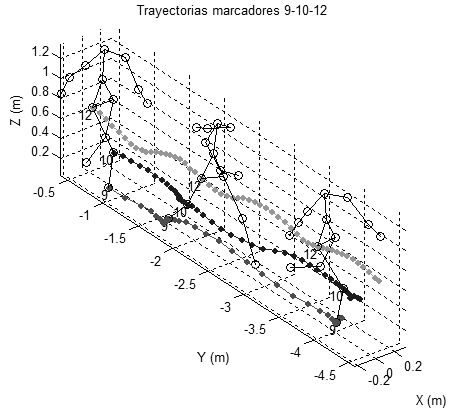
\includegraphics[scale=0.4]{imagenes/Seguimiento/050_Salida_Tracking_13_14_10.png} %\label{trayectorias_marcadores_piernas}
   }	
  \subfloat[Distancia y Angulo entre marcadores de la pierna.]{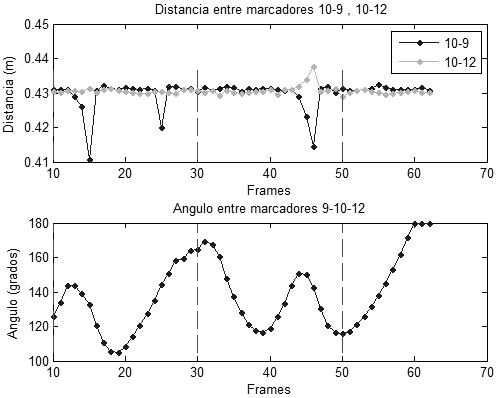
\includegraphics[scale=0.4]{imagenes/Seguimiento/051_Salida_Angulo_Distancia_13_14_10.png}\label{distancia_angulo_marcadores_piernas}}
\caption{Ejemplos de Posibles restricciones en ángulo y distancia, para el caso de la pierna en marcha.}
\label{restricciones_tracking}
\end{figure}